\documentclass{article}

\usepackage[a4paper, left=2cm, right=3cm, top=2.5cm, bottom=2.5cm]{geometry}
\usepackage{amsmath}
\usepackage{amssymb}
\usepackage{dirtree}
\usepackage{url}
\usepackage{hyperref}
\usepackage{graphicx}

\begin{document}

\begin{center}

\section*{LAPORAN TUGAS BESAR 1}

\large{{\textsc{IF2123 Aljabar Linier dan Geometri}}

\textsc{Sistem Persamaan Linier, Determinan, dan Penerapannya}

\textsc{Semester 1 Tahun 2026/2027}

\vspace{0.8cm}

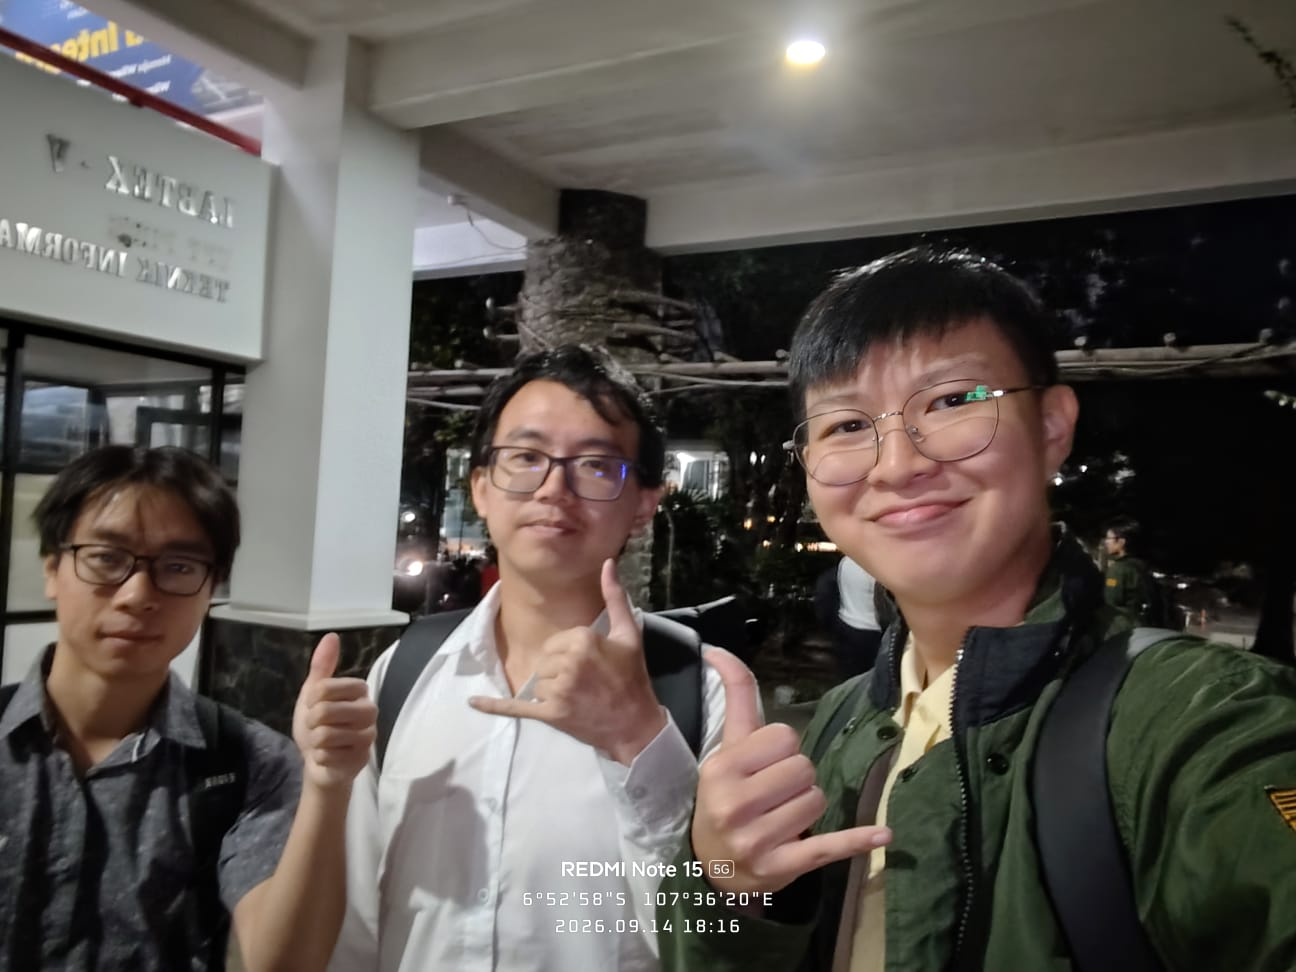
\includegraphics[width=0.8\textwidth]{cover.jpeg}

\vspace{0.8cm}

{\Large\textsc{Anggota Kelompok:}}

\vspace{0.2cm}

\textsc{Laboratorium Ilmu dan Rekayasa Komputasi}

\textsc{Program Studi Teknik Informatika}

\textsc{Sekolah Teknik Elektro dan Informatika}

\textsc{Institut Teknologi Bandung}}

\large{\textsc{Anggota Kelompok: }}

\textsc{Matthew Allen Reynaldo - 13525001}

\textsc{Justin William - 13525042}

\textsc{Kelvin Sebastian Yen - 13525068}

\end{center}

\newpage

\renewcommand{\contentsname}{Daftar Isi}
\tableofcontents

\newpage
\section{Pendahuluan}

Di pelosok Snezhnaya, seorang peneliti muda bernama Mitya tengah berusaha keras memimpin eksperimen krusial berskala raksasa: Proyek Stuzha. Proyek ini digadang-gadang mampu mengendalikan
fluktuasi energi ekstrem di daratan Teyvat. Sayangnya, impian besar tersebut terbentur tembok tebal:
Mitya masih mengandalkan kalkulator saku tua yang sering error tiap kali dipaksa menyelesaikan kalkulasi berdimensi tinggi.

Setelah menjelajahi perpustakaan Sumeru Akademiya hingga menyisir kabar burung ke seantero
Teyvat, Mitya mendengar reputasi kalian sebagai praktisi komputasi dan aljabar linier paling piawai.
Ia pun mengirimkan pesan ke Adventures Guild dan memberikan komisi {\bf perangkat lunak sekelas
Photomath versi Teyvat} yaitu sebuah mesin kalkulasi otomatis yang sanggup melumat sistem matriks
dan persamaan linier rumit demi kelangsungan Proyek Stuzha.
Aljabar linier bukan sekadar teori di atas kertas papirus; ini adalah fondasi komputasi modern yang
menggerakkan simulasi rekayasa, pemodelan aliran energi, analisis data, hingga dinamika sistem kompleks. Agar kalkulasi Proyek Stuzha tidak runtuh di tengah jalan, kalian ditugaskan merancang dan
membangun pustaka (library) komputasi aljabar linier mandiri berbasis bahasa pemrograman {\bf Java} yang
modular, tangguh, dan terdokumentasi rapi.
Pustaka ini nantinya menjadi motor utama di balik alat komputasi Mitya untuk:
\begin{itemize}
    \item{Menyelesaikan {\bf Sistem Persamaan Linier (SPL)}, perhitungan {\bf Determinan}, dan pencarian
{\bf Invers Matriks} guna menganalisis keseimbangan sirkuit daya dan kestabilan instrumen Proyek
Stuzha.}
    \item{Melakukan {\bf Interpolasi Polinomial, Natural Cubic Spline Interpolation, dan regresi Spline}
untuk memetakan jalur transfer energi serta memodelkan kontur data eksperimen secara presisi.}
    \item{{\bf Menerapkan Image Inpainting (Hole Filling) berbasis Persamaan Laplace (Bonus)}
sebagai modul restorasi darurat. Modul ini bertugas merekonstruksi lembar cetak biru dan catatan
eksperimen penting yang kerap berlubang atau hilang secara misterius yang konon merupakan ulah
sabotase usil dari {\bf Renova}.}
\end{itemize}
Melalui tugas besar ini, kalian diharapkan tidak hanya menguasai teori matematika di balik algoritmaalgoritma tersebut, melainkan juga mampu mengonstruksinya menjadi perangkat lunak nyata yang lolos
berbagai skenario uji (test cases) ekstrem.

\noindent{{\bf Tujuan Tugas Besar:}}
\begin{itemize}
    \item{Mengimplementasikan metode penyelesaian SPL, determinan, invers matriks, interpolasi polinomial, Natural Cubic Spline Interpolation, regresi Spline, dan algoritma Image Inpainting berbasis
diskritisasi Persamaan Laplace secara mandiri menggunakan Java.}
    \item{Membangun pustaka (library) aljabar linier yang terstruktur secara modular, bersih, dan terdokumentasi dengan baik. Tidak menggunakan library perhitungan matriks, regresi, atau interpolasi
instan.}
    \item{Menguji keandalan pustaka pada berbagai kasus uji analitis dan restorasi citra, serta menyusun
laporan analisis hasil perhitungannya.}
\end{itemize}

\section{Dasar Teori}
\subsection{Sistem Persamaan Linier}

Sistem Persamaan Linear (SPL) adalah himpunan berhingga dari persamaan-persamaan linear dengan
variabel-variabel yang sama. Bentuk umum dari SPL dengan $m$ persamaan dan $n$ variabel adalah

\[
\left\{
\begin{aligned}
a_{11}x_1 + a_{12}x_2 + a_{13}x_3 + \cdots + a_{1n}x_n &= b_1 \\
a_{21}x_1 + a_{22}x_2 + a_{23}x_3 + \cdots + a_{2n}x_n &= b_2 \\
&\vdots \\
a_{n1}x_1 + a_{n2}x_2 + a_{n3}x_3 + \cdots + a_{nn}x_n &= b_n
\end{aligned}
\right.
\]
\noindent{atau, dalam bentuk perkalian matriks (kiri) dan matriks augmented (kanan)}
\[
\underbrace{
\begin{bmatrix}
a_{11} & a_{12} & \cdots & a_{1n} \\
a_{21} & a_{22} & \cdots & a_{2n} \\
\vdots & \vdots & \ddots & \vdots \\
a_{n1} & a_{n2} & \cdots & a_{nn}
\end{bmatrix}
}_{A}
\underbrace{
\begin{bmatrix}
x_1 \\
x_2 \\
\vdots \\
x_n
\end{bmatrix}
}_{x}
=
\underbrace{
\begin{bmatrix}
b_1 \\
b_2 \\
\vdots \\
b_n
\end{bmatrix}
}_{b}
\quad \longrightarrow \quad
\begin{bmatrix}
a_{11} & a_{12} & \cdots & a_{1n} & b_1 \\
a_{21} & a_{22} & \cdots & a_{2n} & b_2 \\
\vdots & \vdots & \ddots & \vdots & \vdots \\
a_{n1} & a_{n2} & \cdots & a_{nn} & b_n
\end{bmatrix}
\]

Solusi dari SPL dapat berupa solusi tunggal, banyak solusi, atau tidak ada solusi. Metode penyele-
saian yang umum digunakan antara lain eliminasi Gauss, eliminasi Gauss-Jordan, kaidan Cramer, dan
metode matriks balikan.
\subsection{Determinan Matriks}

Determinan adalah sebuah nilai skalar khusus yang dapat dihitung dari elemen-elemen sebuah matriks
persegi. Determinan dari matriks A dinotasikan sebagai det($A$) atau $|A|$. Nilai determinan sangat
krusial karena dapat mengindikasikan apakah matriks tersebut memiliki invers. Beberapa metode untuk
menghitung determinan matriks mencakup metode ekspansi kofaktor dan metode reduksi baris.

\subsection{Invers Matriks}

Invers dari sebuah matriks persegi A adalah matriks $A^{-1}$ yang memenuhi properti $AA^{-1}$ = $A^{-1}A$ =
I, di mana I adalah matriks identitas. Sebuah matriks hanya memiliki invers jika dan hanya jika
determinannya tidak nol (det($A$) $\neq$ 0). Matriks yang memiliki invers disebut matriks invertible atau
non-singular. Perhitungan invers dari suatu matriks dapat dilakukan dengan metode matriks adjoin
maupun metode eliminasi Gauss-Jordan.

\subsection{Interpolasi Polinomial}

Interpolasi polinomial adalah metode untuk menentukan suatu polinomial $P_{n}(x)$ berderajat n yang
melalui n + 1 titik data $(x_0, y_0),(x_1, y_1),\cdots,(x_n, y_n), x_i$ diurutkan dengan $x_0$ terkecil dan $x_n$ terbesar.
Secara umum, polinomial tersebut dapat dituliskan sebagai:

\begin{center}
$P_{n}(x) = a_{0} + a_{1}x + a_{2}x^{2} +\cdots+ a_{n}^{x}$
\end{center}

dengan koefisien $a_{0}, a_{1},\cdots, a_n{n}$ yang ditentukan sedemikian rupa sehingga $P_{n}(x_{perkiraan}) = y_{perkiraan}$
untuk semua nilai $x_{0} < x_{perkiraan} < x_{n}$. Derajat persamaan polinom ditentukan oleh jumlah titik data
yang diberikan dikurangi satu.
Koefisien polinomial dapat dicari dengan menyulihkan titik-titik data ke dalam persamaan polinomial dan menyelesaikan sistem persamaan linear yang dihasilkan dengan metode eliminasi Gauss yang
dijelaskan sebelumnya. Kita dapat menyusun sistem persamaan linear sebagai berikut.

\[
\left\{
\begin{aligned}
& a_0 + a_1x_0 + a_2x_0 + \cdots + a_nx_0^n &= y_0 \\
& a_0 + a_1x_1 + a_2x_1 + \cdots + a_nx_1^n &= y_1 \\
&\vdots \\
& a_0 + a_1x_n + a_2x_n + \cdots + a_nx_n^n &= y_n
\end{aligned}
\right.
\]

Persamaan-persamaan di atas dapat dipetakan menjadi sebuah permasalahan sistem persamaan linear, sehingga dapat diselesaikan dengan menggunakan metode eliminasi Gauss untuk menyelesaikan sistem tersebut dan menemukan koefisien polinomial $a_0, a_1,\cdots, a_n$. Dari polinom $P_{n}(x)$ yang dibentuk dengan koefisien tersebut, kita dapat memperkirakan nilai y untuk nilai x yang berada di antara
titik-titik data yang diberikan (interpolasi) maupun di luar titik-titik data tersebut (ekstrapolasi).

\subsection{Natural Cubic Spline Interpolation}

{\it Interpolasi Spline Kubik (Cubic Spline Interpolation)} adalah metode untuk melakukan interpolasi fungsi berderajat tiga yang kontinu dalam suatu rentang koordinat berdasarkan titik koordinat yang diketahui. Bentuk kubik standar dalam setiap rentang adalah \cite{anton}:
\[
S{(x)} = a_{n-1}(x - x_{n-1})^3 + b_{n-1}(x - x_{n-1})^2 + c_{n-1}(x - x_{n-1}) + d_{n-1} \qquad x_{n-1} \leq x \leq x_n
\]
Nilai masing-masing koefisien didefinisikan sebagai berikut:
\[
a_i = \frac{(M_{i+1} - M_i)}{6h} \qquad
b_i = \frac{M_i}{2} \qquad
c_i = \frac{(y_{i+1} - y_i)}{h} - \frac{h[M_{i+1} + 2M_i]}{6} \qquad d_i = y_i
\]
dengan i = 1, 2, \ldots, n - 1, dengan $M_i$ = $S"(xi)$ untuk i = 1, 2, \ldots, n.
Pada interpolasi splina kubik natural, turunan kedua pada koordinat ujung kiri dan kanan bernilai 0, yaitu $M_1$ = 0 dan $M_n$ = 0. Syarat ini ditetapkan agar nilai M dapat dicari. Untuk mendapatkan nilai $M_1$, $M_2$, ... $M_n$, dilakukan substitusi persamaan $a_i$, $b_i$, dan $c_i$ ke dalam persamaan turunan pertama dalam rentang [$x_1$, $x_n$]:
\[
3a_{n-2}h^2 + 2b_{n-2}h + c_{n-2} = c_{n - 1}
\]
Proses substitusi akan menghasilkan n - 2 buah persamaan dalam bentuk:
\[
M_{n-2} + 4_{Mn-1} + M_n = \frac{6(y_1 - 2y_2 + y_3)}{h^2}
\]
Jika sistem persamaan linear tersebut disusun menjadi sebuah matriks, maka akan terbentuk suatu matriks tridiagonal dengan format sebagai berikut:
\[
\begin{bmatrix}
    1 & 4 & 1 & 0 & \cdots & 0 & 0 & 0 & 0 \\
    0 & 1 & 4 & 1 & \cdots & 0 & 0 & 0 & 0 \\
    0 & 0 & 1 & 4 & \cdots & 0 & 0 & 0 & 0 \\
    \vdots & \vdots & \vdots & \vdots  & &  \vdots & \vdots & \vdots & \vdots \\
    0 & 0 & 0 & 0 & \cdots & 4 & 1 & 0 & 0 \\
    0 & 0 & 0 & 0 & \cdots & 1 & 4 & 1 & 0 \\
    0 & 0 & 0 & 0 & \cdots & 0 & 1 & 4 & 1 \\
\end{bmatrix}
\begin{bmatrix}
    M_1 \\
    M_2 \\ 
    M_3 \\
    M_4 \\
    \vdots \\
    M_{n-3} \\
    M_{n-2} \\
    M_{n-1} \\
    M_{n} 
\end{bmatrix} = \frac{6}{h^2} 
\begin{bmatrix}
    y_1 - 2y_2 + y_3 \\
    y_2 - 2y_3 + y_4 \\
    y_3 - 2y_4 + y_5 \\
    \vdots \\
    y_{n-4} - 2y_{n-3} + y_{n-2} \\
    y_{n-3} - 2y_{n-2} + y_{n-1} \\
    y_{n-2} - 2y_{n-1} + y_{n}
\end{bmatrix}
\]
Setelah diperoleh sistem persamaan linear berbentuk matriks tridiagonal n - 2 x n, telah diketahui bahwa syarat batas natural menetapkan nilai $M_1$ = 0 dan $M_n$ = 0. Oleh karena itu, matriks tridiagonal dapat disederhanakan menjadi matriks n - 2 x n -2 sebagai berikut:
\[
\begin{bmatrix}
    4 & 1 & 0 & \cdots & 0 & 0 & 0\\
    1 & 4 & 1 & \cdots & 0 & 0 & 0 \\
    0 & 1 & 4 & \cdots & 0 & 0 & 0 \\
    \vdots & \vdots & \vdots  & &  \vdots & \vdots & \vdots & \\
    0 & 0 & 0 & \cdots & 4 & 1 & 0 \\
    0 & 0 & 0 & \cdots & 1 & 4 & 1 \\
    0 & 0 & 0 & \cdots & 0 & 1 & 4 \\
\end{bmatrix}
\begin{bmatrix}
    M_2 \\ 
    M_3 \\
    M_4 \\
    \vdots \\
    M_{n-3} \\
    M_{n-2} \\
    M_{n-1} \\
\end{bmatrix} = \frac{6}{h^2} 
\begin{bmatrix}
    y_1 - 2y_2 + y_3 \\
    y_2 - 2y_3 + y_4 \\
    y_3 - 2y_4 + y_5 \\
    \vdots \\
    y_{n-4} - 2y_{n-3} + y_{n-2} \\
    y_{n-3} - 2y_{n-2} + y_{n-1} \\
    y_{n-2} - 2y_{n-1} + y_{n}
\end{bmatrix}
\]


\subsection{Splines Regression}
\textit{Splines Regression} adalah metode regresi yang memprediksi nilai y dari suatu input x. Polinomial kubik memiliki bentuk: 
\[
h_0(x) = 1, \qquad 
h_1(x) = x, \qquad
h_2(x) = x^2, \qquad
h_3(x) = x^3
\]
Untuk splina kubik, fungsi regresi menggabungkan polinomial global dengan \textit{truncated power basis} sehingga menghasilkan fungsi regresi baru:
\[
f(x) = \sum_{j = 0}^{3+K} \beta_jh_j(x) = \beta_0 + \beta_1x + \beta_2x^2 + \beta_3x^3 + \sum_{k = 3}^{K} \beta_{3+k}(x-\xi_k)^3_+
\]
atau jika disusun ke dalam bentuk matriks:
\[
X=
\begin{bmatrix}
1 & x_1 & x_1^2 & x_1^3 &
(x_1-\xi_1)_+^3 &
(x_1-\xi_2)_+^3 &
\cdots &
(x_1-\xi_K)_+^3
\\
1 & x_2 & x_2^2 & x_2^3 &
(x_2-\xi_1)_+^3 &
(x_2-\xi_2)_+^3 &
\cdots &
(x_2-\xi_K)_+^3
\\
\vdots & \vdots & \vdots & \vdots &
\vdots & \vdots & \ddots & \vdots
\\
1 & x_N & x_N^2 & x_N^3 &
(x_N-\xi_1)_+^3 &
(x_N-\xi_2)_+^3 &
\cdots &
(x_N-\xi_K)_+^3
\end{bmatrix}
\]
dengan K adalah jumlah knot dalam batas. Namun, nilai dari setiap perhitungan $(x-\xi_k)_+^3$ perlu ditentukan terlebih dulu melalui fungsi piecewise berikut:
\[
(x-\xi_k)_+^3 = 
\begin{cases}
    (x-\xi_k)^3, & x > \xi_k \\
    0, &x \leq \xi_k 
\end{cases}
\]
Menggunakan matrix tersebut, nilai koefisien $\beta$ dapat diestimasi. Dikutip dari Hastie, jika diasumsikan X memiliki kolom \textit{rank} penuh, maka jika turunan pertama ditetapkan sebagai 0, diperoleh \cite{hastie}
\[
X^T(y-X\beta) = 0
\]
yang menghasilkan persamaan normal:
\[
(X^TX)\beta = X^Ty
\]
Dari persamaan normal, solusi untuk $\beta$ didapatkan melalui manipulasi bentuk:
\[
\hat{\beta} = (X^TX)^{-1}X^Ty
\]

\subsection{Diskritisasi Persamaan Laplace dan Algoritma Gauss-Seidel}
Persamaan Laplace pada bidang 2-dimensi merupakan persamaan diferensial kontinu dengan bentuk sebagai berikut  \cite{chapra}:
\[
\triangledown^2 = \frac{\partial^2 P}{\partial x^2} + \frac{\partial^2 P}{\partial y^2} = 0
\]
Setiap komponen dari persamaan Laplace dalam ruang 2-dimensi didefinisikan sebagai:
\[
\frac{\partial^2 P}{\partial x^2} = \frac{P_{i+1,j} - 2P_{i,j} + P_{i-1,j}}{\Delta x^2} \qquad \frac{\partial^2 P}{\partial y^2} = \frac{P_{i,j+1} - 2P_{i,j} + P_{i,j-1}}{\Delta y^2}
\]
Jika nilai dari masing-masing komponen disubstitusikan ke dalam persamaan Laplace, maka akan diperoleh persamaan::
\[
\frac{P_{i+1,j} - 2P_{i,j} + P_{i-1,j}}{\Delta x^2} + \frac{P_{i,j+1} - 2P_{i,j} + P_{i,j-1}}{\Delta y^2} = 0
\]
Dalam suatu grid 2-dimensi, diasumsikan bahwa jarak antar titik x dan jarak antar titik y sama, sehingga dapat ditulis $\Delta x^2$ = $\Delta y^2$. Maka dari itu, persamaan dapat disederhanakan menjadi:
\[
P_{i+1,j} + P_{i-1,j} + {P_{i,j+1} + P_{i,j-1} - 4P_{i,j}  = 0
\]
Persamaan tersebut dapat disederhanakan lebih lanjut untuk menghitung nilai suatu koordinat pada grid:
\[
P_{i,j} = \frac{P_{i+1,j} + P_{i-1,j} + P_{i,j+1} + P_{i,j-1}}{4}
\]
Metode Gauss-Seidel adalah metode penyelesaian iteratif yang dapat digunakan untuk mendapatkan solusi SPL. Berbeda dari metode Jacobi, setelah nilai dari suatu variabel yang tidak diketahui diperbarui, nilai tersebut tidak digunakan pada iterasi berikutnya, melainkan pada persamaan berikutnya di iterasi yang sama. Contoh penggunaan dari metode Gauss-Seidel adalah sebagai berikut:

Iterasi pertama \cite{munir}:

\begin{align*}
x_1^{(1)} = \frac{b_1 - a_{12}x_2^{(0)} - a_{13}x_3^{(0)} - a_{14}x_4^{(0)}}{a_{11}} \\
x_2^{(1)} = \frac{b_1 - a_{21}x_1^{(1)} - a_{23}x_3^{(0)} - a_{24}x_4^{(0)}}{a_{22}} \\
x_3^{(1)} = \frac{b_3 - a_{31}x_1^{(1)} - a_{32}x_3^{(1)} - a_{34}x_4^{(0)}}{a_{33}}\\
x_4^{(1)} = \frac{b_4 - a_{41}x_1^{(1)} - a_{42}x_3^{(1)} - a_{43}x_3^{(1)}}{a_{44}}
\end{align*}

Dapat dilihat bahwa $x_2$ langsung menggunakan nilai $x_1$ yang sudah diperbarui. Dengan menerapkan galat, penggunaan algoritma Gauss-Seidel akan konvergen dan berhenti setelah mencapai batas yang ditentukan.


\section{Implementasi}

\subsection{Struktur Kelas}
Struktur kelas dalam program ini adalah sebagai berikut:
\dirtree{%
.1 src/.
.2 main/.
.3 java/.
.4 algeo/.
.5 modules/.
.6 CramerRule.java/.
.6 CubicSplineInterpolation.java/.
.6 GaussElim.java/.
.6 GaussJordanElim.java/.
.6 ImageRestoration.java/.
.6 InverseMethod.java/.
.6 Matrix.java/.
.6 OBE.java/.
.6 PolinomialInterpolation.java/.
.6 SplineRegression.java/.
.6 Utilities.java/.
.1 test/.
.2 .gitkeep/.
.1 gitignore/.
.1 pom.xml/.
.1 README.md/.
}
\subsection{Arsitektur Pustaka}

\noindent{Struktur kelas pada pustaka aljabar linier ini dirancang secara modular untuk memisahkan fungsi setiap komponen. Berikut adalah kelas-kelas yang sudah dirancang:}

\subsubsection{Matrix}

\noindent{Matrix merupakan kelas yang digunakan untuk merepresentasikan struktur data matriks. Kelas ini menyimpan jumlah baris, jumlah kolom, serta elemen-elemen matriks dalam bentuk array dua dimensi bertipe \texttt{double}.}

\begin{enumerate}

    \item{\texttt{Matrix}: konstruktor yang digunakan untuk membuat matriks baru dengan ukuran baris dan kolom tertentu. Seluruh elemen matriks diinisialisasi dengan nilai awal 0.}

\end{enumerate}


\subsubsection{OBE}

\noindent{OBE atau Operasi Baris Elementer merupakan kelas yang berfungsi untuk melakukan operasi baris elementer pada matriks. Kelas ini memiliki beberapa metode atau fungsi yang dapat digunakan untuk melakukan operasi seperti:}

\begin{enumerate}

    \item{\texttt{swapRow}: menukar posisi dua baris pada matriks.}

    \item{\texttt{multiplyRow}: mengalikan seluruh elemen suatu baris dengan suatu konstanta.}

    \item{\texttt{addMultipleRow}: menambahkan suatu baris dengan kelipatan dari baris lain.}

    \item{\texttt{findPivotRow}: mencari indeks baris dengan nilai absolut elemen terbesar pada kolom tertentu sebagai baris pivot.}

\end{enumerate}


\subsubsection{Utilities}

\noindent{Utilities merupakan kelas yang menyediakan berbagai fungsi utilitas untuk melakukan operasi dasar dan pemeriksaan terhadap matriks. Kelas ini digunakan oleh berbagai modul lain dalam program. Metode-metode yang tersedia antara lain:}

\begin{enumerate}

    \item{\texttt{createMatrix}: membuat matriks baru dengan ukuran baris dan kolom tertentu.}

    \item{\texttt{showMatrix}: menampilkan elemen-elemen matriks ke layar dengan format tiga angka di belakang koma.}

    \item{\texttt{setMatrixElement}: mengubah nilai elemen matriks pada posisi baris dan kolom tertentu.}

    \item{\texttt{getMatrixElement}: mengambil nilai elemen matriks pada posisi baris dan kolom tertentu.}

    \item{\texttt{isSquareMatrix}: memeriksa apakah suatu matriks merupakan matriks persegi.}

    \item{\texttt{isMatrixIdentity}: memeriksa apakah suatu matriks merupakan matriks identitas.}

    \item{\texttt{isValidMatrixAddSub}: memeriksa apakah dua matriks memiliki ukuran yang sama sehingga dapat dijumlahkan atau dikurangkan.}

    \item{\texttt{isValidMatrixMul}: memeriksa apakah dua matriks memenuhi syarat untuk dilakukan perkalian matriks.}

    \item{\texttt{transposeMatrix}: menghasilkan transpose dari suatu matriks.}

    \item{\texttt{matrixMultiplication}: melakukan perkalian antara dua matriks jika dimensinya memenuhi syarat.}

    \item{\texttt{matrixAddition}: melakukan penjumlahan dua matriks yang memiliki ukuran sama.}

    \item{\texttt{matrixSubtraction}: melakukan pengurangan dua matriks yang memiliki ukuran sama.}

    \item{\texttt{copyMatrix}: membuat salinan matriks dengan ukuran yang sama dan menyalin elemen-elemennya.}

    \item{\texttt{createMatrixIdentity}: membuat matriks identitas dengan ordo tertentu.}

    \item{\texttt{replaceColumn}: membuat salinan matriks dengan mengganti salah satu kolom menggunakan elemen dari suatu vektor.}

    \item{\texttt{subMatrix}: membuat submatriks dengan menghapus satu baris dan satu kolom dari matriks asal.}

    \item{\texttt{Determinant}: menghitung determinan matriks persegi menggunakan metode ekspansi kofaktor secara rekursif.}

    \item{\texttt{power}: menghitung nilai perpangkatan bilangan bulat secara rekursif.}

    \item{\texttt{Cofactor}: membentuk matriks kofaktor dari suatu matriks.}

    \item{\texttt{ScalarMatrixMul}: mengalikan seluruh elemen matriks dengan suatu skalar.}

    \item{\texttt{InverseMatrix}: menghitung invers matriks menggunakan matriks kofaktor, transpose kofaktor, dan nilai determinan.}

    \item{\texttt{DeterminantOBE}: menghitung determinan matriks menggunakan operasi baris elementer.}

    \item{\texttt{InverseMatrixAugmented}: menghitung invers matriks menggunakan metode matriks augmented dan operasi Gauss-Jordan.}

\end{enumerate}


\subsubsection{GaussElim}

\noindent{GaussElim merupakan kelas yang digunakan untuk menyelesaikan sistem persamaan linear menggunakan metode eliminasi Gauss. Kelas ini juga menangani klasifikasi jenis solusi sistem persamaan linear, yaitu solusi tunggal, solusi tak hingga, dan tidak memiliki solusi. Metode yang tersedia antara lain:}

\begin{enumerate}

    \item{\texttt{formatNumber}: mengubah nilai \texttt{double} menjadi representasi string dan menghilangkan bagian desimal apabila nilainya merupakan bilangan bulat.}

    \item{\texttt{findPivotColumnAfterREF}: mencari kolom pivot pada setiap baris setelah matriks diubah menjadi bentuk eselon baris.}

    \item{\texttt{isPivotColumn}: memeriksa apakah suatu kolom merupakan kolom pivot.}

    \item{\texttt{toRowEchelonFormMatrix}: mengubah matriks menjadi bentuk eselon baris menggunakan eliminasi Gauss dan operasi baris elementer.}

    \item{\texttt{backSubstitution}: menentukan nilai variabel dengan melakukan substitusi balik dari matriks berbentuk eselon baris.}

    \item{\texttt{createParametricSolution}: membentuk representasi solusi parametrik untuk sistem persamaan linear yang memiliki solusi tak hingga.}

    \item{\texttt{solveByGaussElim}: menyelesaikan sistem persamaan linear dengan eliminasi Gauss dan menentukan jenis solusinya.}

\end{enumerate}


\subsubsection{GaussJordanElim}

\noindent{GaussJordanElim merupakan kelas yang digunakan untuk menyelesaikan sistem persamaan linear menggunakan metode eliminasi Gauss-Jordan. Kelas ini menghasilkan bentuk eselon baris tereduksi dan menentukan jenis solusi dari sistem persamaan linear.}

\begin{enumerate}

    \item{\texttt{toReducedRowEchelonFormMatrix}: mengubah suatu matriks menjadi bentuk eselon baris tereduksi menggunakan eliminasi Gauss-Jordan.}

    \item{\texttt{solveByGaussJordan}: menyelesaikan sistem persamaan linear menggunakan bentuk eselon baris tereduksi serta menentukan apakah sistem memiliki solusi tunggal, solusi tak hingga, atau tidak memiliki solusi.}

\end{enumerate}


\subsubsection{CramerRule}

\noindent{CramerRule merupakan kelas yang digunakan untuk menyelesaikan sistem persamaan linear menggunakan aturan Cramer. Metode ini menggunakan nilai determinan matriks koefisien dan matriks yang kolomnya digantikan dengan vektor konstanta.}

\begin{enumerate}

    \item{\texttt{cramerRule}: menghitung solusi sistem persamaan linear menggunakan aturan Cramer dengan mengganti setiap kolom matriks koefisien menggunakan vektor konstanta dan menghitung perbandingan determinannya.}

\end{enumerate}


\subsubsection{InverseMethod}

\noindent{InverseMethod merupakan kelas yang digunakan untuk menyelesaikan sistem persamaan linear menggunakan metode invers matriks. Kelas ini memisahkan matriks augmented menjadi matriks koefisien dan vektor konstanta sebelum menghitung solusi.}

\begin{enumerate}

    \item{\texttt{splitAugmentMatrix}: memisahkan matriks augmented menjadi matriks koefisien A dan vektor konstanta b.}

    \item{\texttt{inverseMethod}: menghitung solusi sistem persamaan linear dengan menggunakan hubungan \(x = A^{-1}b\), setelah memastikan matriks A berbentuk persegi dan memiliki invers.}

\end{enumerate}


\subsubsection{PolinomialInterpolation}

\noindent{PolinomialInterpolation merupakan kelas yang digunakan untuk melakukan interpolasi polinomial berdasarkan sekumpulan titik data. Interpolasi dibentuk dengan menggunakan matriks Vandermonde dan diselesaikan menggunakan eliminasi Gauss.}

\begin{enumerate}

    \item{\texttt{createAugmentedMatrix}: menggabungkan matriks koefisien A dengan vektor konstanta b menjadi suatu matriks augmented.}

    \item{\texttt{Interpolate}: membentuk matriks Vandermonde berdasarkan titik-titik yang diberikan, kemudian menyelesaikan sistem persamaan linear untuk mendapatkan koefisien polinomial interpolasi.}

\end{enumerate}


\subsubsection{CubicSplineInterpolation}

\noindent{CubicSplineInterpolation merupakan kelas yang digunakan untuk melakukan interpolasi spline kubik berdasarkan sekumpulan titik data. Data diurutkan berdasarkan nilai x kemudian dibentuk sistem persamaan linear untuk memperoleh koefisien persamaan yang dipakai untuk membangun persamaan pada setiap interval.} 

 \begin{enumerate} 

     \item{\texttt{interpolate}: menerima sejumlah titik data, mengurutkannya berdasarkan nilai x, membentuk matriks tridiagonal spline kubik, menyelesaikan sistem persamaan menggunakan Gauss-Jordan, kemudian menghitung koefisien spline untuk setiap interval. \cite{g4g} Setelah koefisien spline didapatkan, dibangun persamaan interpolasi untuk setiap interval. Program akan menghasilkan beberapa luaran, antara lain nilai turunan pada setiap titik temu interval, persamaan setiap interval dan domainnya. Terakhir, program akan meminta input nilai x untuk interpolasi nilai y}  

    \item{\texttt{main}: merupakan titik awal program untuk menjalankan proses interpolasi fungsi dan nilai.}

\end{enumerate}


\subsubsection{SplineRegression}

\noindent{SplineRegression merupakan kelas yang digunakan untuk melakukan regresi spline berdasarkan data yang diberikan pengguna. Program membentuk fungsi regresi dari basis polinomial dan \textit{truncated power basis} berdasarkan knot yang ditentukan, kemudian menghitung koefisien regresi menggunakan pendekatan kuadrat terkecil.}

\begin{enumerate}

    \item{\texttt{calculate}: menerima jumlah data dan jumlah knot, membentuk matriks basis regresi spline, menghitung matriks normal menggunakan \(X^T X\) dan \(X^T y\), kemudian menyelesaikan sistem persamaan menggunakan eliminasi Gauss-Jordan untuk memperoleh koefisien regresi. Luaran yang dihasilkan adalah daftar koefisien regresi, daftar posisi knot, persamaan regresi, dan hasil prediksi fungsi setelah menerima input}

    \item{\texttt{main}: merupakan titik awal program untuk menjalankan proses perhitungan regresi spline.}

\end{enumerate}


\subsubsection{ImageRestoration}

\noindent{ImageRestoration merupakan kelas yang digunakan untuk melakukan restorasi gambar dengan memperkirakan nilai piksel yang rusak berdasarkan nilai piksel tetangganya. Program menggunakan gambar mask untuk menentukan posisi piksel yang perlu direstorasi dan melakukan iterasi hingga galat memenuhi batas yang ditentukan.}

\begin{enumerate}

    \item{\texttt{jalankan}: menerima path gambar asli, path gambar mask, dan path keluaran. Mengubah mask menjadi matriks untuk membaca piksel rusak, membuat array kosong sebagai kanvas gambar untuk menyalin warna yang tidak rusak dari gambar asli, memperbarui nilai piksel rusak menggunakan rata-rata empat piksel tetangga dengan melakukan iterasi hingga galat terbesar lebih kecil dari galat maksimum, menyimpan hasil restorasi dalam format PNG, dan mengembalikan galat terbesar sebelum iterasi berhenti}

    \item{\texttt{main}: merupakan titik awal program untuk menjalankan proses restorasi gambar.}

\end{enumerate}

\subsection{Alur Program}
\begin{itemize}
\item{Program mulai berjalan dan meminta input angka untuk memilih modul yang ingin digunakan. Jika input tidak valid, pengguna akan diminta untuk kembali memberikan input}
\item{Program meminta input yang diperlukan untuk melakukan perhitungan sesuai modulnya melalui input langsung atau direktori file .txt/.png)}
\item{Pengguna memasukkan input yang kemudian diterima program. Program akan mengolah input agar dapat digunakan dan melakukan perhitungan sesuai input yang diberikan.}
\item{Program akan mencetak output hasil perhitungan (output di terminal atau file .txt, image inpainting akan menghasilkan file .png)}
\end{enumerate}
\section{Eksperimen}

\section{Penutup}
Spek tugas besar, antara lain metode penyelesaian SPL, determinan dan invers matriks, interpolasi polynomial, Natural Cubic Spline Interpolation, regresi Spline, serta Image Inpainting melalui diskritisasi Persamaan Laplace berhasil diimplementasikan secara mandiri tanpa library perhitungan dalam bahasa pemrograman Java. Pustaka aljabar linier telah dibuat sesuai spek, yakni terstruktur secara modular, bersih, dan terdokumentasi dengan baik. Pustaka telah diuji melalui beberapa uji kasus, dapat menghasilkan luaran, serta telah dibuatkan laporan analisis hasil perhitungan. \\
Kelebihan dari sistem yang telah dibangun: 
\begin{enumerate}

    \item{Melakukan perhitungan dengan cepat dan tepat}
    \item{Mudah digunakan}
    \item{CLI yang menampilkan output dengan lengkap, jelas, dan rapi}
    \item{Input bisa langsung di terminal atau melalui direktori file}

\end{enumerate}
Namun, sistem ini masih memiliki kekurangan, antara lain:
\begin{enumerate}

    \item{Tidak ada GUI yang menarik}
    \item{Tidak ada grafik yang menampilkan hasil interpolasi dan regresi}
    \item{Potensi kasus ujung yang belum ditemukan}
    \item{Penulisan kode berantakan}
    \item{Dokumentasi kode minimal}
    \item{Input manual pada terminal kurang nyaman digunakan}

\end{enumerate}

\section{Daftar Pustaka}
\begin{thebibliography}{9}

\bibitem{anton}
H. Anton and C. Rorres, \textit{Elementary Linear Algebra: Applications Version}, 11th ed. Hoboken, NJ: Wiley, 2013.

\bibitem{munir}
R. Munir, \textit{Metode Numerik}, Ed. Rev. 5. Bandung, Indonesia: Penerbit Informatika, 2021.

\bibitem{chapra}
S. C. Chapra and R. P. Canale, \textit{Numerical Methods for Engineers}, 7th ed. New York, NY: McGraw-Hill Education, 2015.

\bibitem{hastie}
T. Hastie, R. Tibshirani, and J. Friedman, \textit{The Elements of Statistical Learning: Data Mining, Inference, and Prediction}, 2nd ed. New York, NY: Springer, 2009.

\bibitem{g4g}
``Cubic Spline Interpolation,'' geeksforgeeks.org, \url{https://www.geeksforgeeks.org/machine-learning/cubic-spline-interpolation/}. *Accessed: 2-Oct-2026.

\bibitem{javaio}

GeeksforGeeks, ``Java IO Tutorial,'' \textit{GeeksforGeeks}, 2025. [Online]. Available: \url{https://www.geeksforgeeks.org/java/java-io-tutorial/}. [Accessed: 2-Oct-2026].

\bibitem{accessmodifiers}

GeeksforGeeks, ``Public vs Private Access Modifiers in Java,'' \textit{GeeksforGeeks}, 2021. [Online]. Available: \url{https://www.geeksforgeeks.org/java/public-vs-private-access-modifiers-in-java/}. [Accessed: 2-Oct-2026].

\bibitem{exceptionjava}

GeeksforGeeks, ``Java Exception Handling,'' \textit{GeeksforGeeks}, 2026. [Online]. Available: \url{https://www.geeksforgeeks.org/java/exceptions-in-java/}. [Accessed: 2-Oct-2026].

\bibitem{maven}

GeeksforGeeks, ``Maven Tutorial,'' \textit{GeeksforGeeks}, 2026. [Online]. Available: \url{https://www.geeksforgeeks.org/advance-java/maven-tutorial/}. [Accessed: 2-Oct-2026].

\end{thebibliography}

\section{Lampiran}

\noindent{Tautan repositori: {\href{https://github.com/Justin273532/algeo26-tb1-kondisikansajakeluargaku\}{algeo26-tb1-kondisikansajakeluargaku}}}

\noindent{LaTeX digunakan untuk membuat dokumen yang rapi. Tautan lokasi berkas LaTeX: {\href{https://github.com/Justin273532/algeo26-tb1-kondisikansajakeluargaku}{algeo26-tb1-kondisikansajakeluargaku}}}

\newpage

\noindent
Tugas ini disusun sepenuhnya tanpa bantuan kecerdasan buatan
(\textit{Generative AI}), melainkan hasil pemikiran dan analisis mandiri.

\vspace{1cm}

\begin{flushright}


\includegraphics[width=3cm]{ttdketuakelompok.jpeg}

\textit{Matthew Allen Reynaldo}\\
13525001

\vspace{0.8cm}


\includegraphics[width=3cm]{ttdanggota2.png}

\textit{Justin William}\\
13525042

\vspace{0.8cm}


\includegraphics[width=3cm]{ttdanggota1.jpeg}

\textit{Kelvin Sebastian Yen}\\
13525068

\end{flushright}

\end{document}